\chapter{Agenti Razionali e Architetture}

\section{Credenze, Desideri e Intenzioni}

\dfn{Sistema Intenzionale}{
  Un sistema intenzionale è un sistema il cui comportamento può essere previsto dal metodo di attribuzione di credenze, di desideri e di acume razionale.
}

\nt{Per McCarthy, in alcuni casi si possono attribuire posizioni intenzionali a sistemi informatici.}

\clm{}{}{
  \begin{itemize}
    \item Più si sa di un sistema meno si fa affidamento a spiegazioni animistiche. 
    \item Con sistemi complessi una spiegazione meccanica potrebbe non essere praticabile.
  \end{itemize}
}

\dfn{Intenzioni e Astrazioni}{
  Più i sistemi di calcolo diventano complessi più si ha bisogno di astrazioni e metafore per spiegare il loro funzionamento. Le posizioni intenzionali sono una tale astrazione.
}

\nt{Le nozioni intenzionali sono quindi astrazioni che forniscono un modo semplice e familiare per descrivere, spiegare e prevedere il comportamento di sistemi complessi.}

\paragraph{I più importanti sviluppi sono basati su astrazioni:}

\begin{itemize}
  \item Procedure e funzioni. 
  \item Tipi di dati astratti (bloat). 
    \item Oggetti. 
    \item Agenti intelligenti e sistemi intenzionali. 
\end{itemize}

\subsection{Ragionamento su Azioni}

\dfn{Pratical Reasoning}{
  Il pratical reasoning è il ragionamento sulle azioni, sul processo di capire cosa fare.
}

\nt{Si distingue da theoretical reasoning che riguarda le credenze.}

\paragraph{Il pratical reasoning consiste in:}

\begin{itemize}
  \item \fancyglitter{Deliberazione}: decidere quale stato di cose vogliamo raggiungere. 
  \item \fancyglitter{Pianificazione} (menas-ends reasoning/planning): decidere come raggiungere questi stati di cose.
\end{itemize}

\nt{Dopo aver ottenuto un piano un agente tenterà di eseguirlo.}

\clm{}{}{
  \begin{itemize}
    \item Il calcolo è una risorsa preziosa per gli agenti, un agente deve controllare il suo ragionamento. 
    \item Gli agenti non possono deliberare a tempo indeterminato, a un certo punto devono smettere di deliberare e, dopo aver scelto uno stato di cose, impegnarsi per raggiungerlo.
  \end{itemize}
}

\cor{Intenzioni}{
  Ci riferiamo allo stato di cose che un agente ha scelto e al quale si impegna come le sue intenzioni.
}

\nt{Il ruolo delle intenzioni è quello di \fancyglitter{favorire la proattività}, ossia portare all'azione.}

\paragraph{Conseguenze:}

\begin{itemize}
  \item Persistenza delle azioni: se si adotta un'intenzione allora si deve insistere su essa e tentare di realizzarla. Se la motivazione cessa di esistere è razionale abbandore l'intenzione. 
  \item Le intenzioni vincolano il futuro pratical reasoning.
\end{itemize}

\paragraph{Intenzioni nel pratical reasoning:}

\begin{enumerate}
  \item Ci si aspetta che gli agenti trovino i modi per realizzare le loro intenzioni. 
  \item Le intenzioni forniscono un \fancyglitter{filtro} per l'adozione di altre intenzioni, che non devono entrare in conflitto. 
  \item Gli agenti monitorano il successo delle loro intenzioni e sono inclini a \fancyglitter{riprovare} se i loro tentativi falliscono. 
  \item  Gli agenti credono che le loro intenzioni siano possibili\footnote{Gli agenti sono come Naruto che vuole diventare Hokage.}. 
  \item Gli agenti non credono che non realizzeranno le loro intenzioni\footnote{Gli agenti sono come Naruto che vuole diventare Hokage pt. 2.}. 
  \item Nelle giuste circostanze gli agenti credono che realizzeranno le loro intenzioni. 
  \item Gli agenti non devono necessariamente avere intenzioni su tutti gli effetti collaterali delle loro intenzioni.
\end{enumerate}

\clm{}{}{
\begin{itemize}
  \item Il problema di avere l'intenzione di realizzare qualcosa credendo che non sia possibile è noto come \fancyglitter{intention-belief inconsistency} e non è razionale. (punto 5)
  \item Il problema di avere l'intenzione di realizzare qualcosa senza credere che la realizzeranno è noto come \fancyglitter{intention-belief incompleteness} ed è una proprietà accettabile per gli agenti razionali. (punto 6)
  \item Il problema al punto 7 è noto come \fancyglitter{package deal}. 
  \end{itemize}
}

\subsection{Modellazione Logica di Agenti BDI}

\begin{itemize}
  \item La logica riguarda principalmente il \fancyglitter{rational balance} relativo a beliefs, goals, plans, intentions, commitments e azioni di agenti autonomi. 
  \item L'obiettivo principale è di esplorare le reazioni che le intenzioni hanno nel mantenere questo bilanciamento. 
  \item Questo deve essere analizzato con \fancyglitter{beliefs}, \fancyglitter{desires} e \fancyglitter{intentions} (BDI).
\end{itemize}

\paragraph{La logica di Cohen e Levesque ha 4 operatori modali principali:}

\begin{itemize}
  \item $(BEL\: i\: \phi)$: l'agente $i$ crede $\phi$.
  \item $(GOAL\: i\: \phi)$: l'agente $i$ ha il goal (desire) $\phi$. 
  \item $(HAPPENS\:\alpha)$: l'azione $\alpha$ occorre al passo successivo. 
  \item $(DONE\: \alpha)$ l'azione $\alpha$ è appena occorsa.
\end{itemize}

\nt{Un'azione $\alpha$ può essere un evento primitivo oppure complesso. L'intenzione non è un operatore primitivo, ma può essere derivato.}

\paragraph{Successivamente viene proposta un'altra logica, da Rao e Georgeff (BDI):}

\begin{itemize}
  \item Ci sono tre modalità: $BEL$, $GOAL$ e $INTEND$. 
  \item I mondi sono strutture temporali branching time. 
\end{itemize}

\paragraph{È possibile descrivere commitments diversi:}

\begin{itemize}
  \item Agente \fancyglitter{blindy committed} (fanatical): mantiene le sue intenzioni finché non arriva a credere di averle soddisfatte. $$INTEND(AF\:\phi) \Rightarrow A(INTEND(AF\:\phi) \cup BEL(\phi))$$
  \item Agente \fancyglitter{Single-minded committed}: mantiene le sue intenzioni finché crede che queste possano essere realizzabili.  $$INTEND(AF\:\phi) \Rightarrow A(INTEND(AF\:\phi) \cup (BEL(\phi) \lor \neg BEL(EF\:\phi)))$$
  \item Agente \fancyglitter{open-minded}: mantiene le sue intenzioni finché queste intenzioni sono ancora i suoi goals. $$INTEND(AF\:\phi) \Rightarrow A(INTEND(AF\:\phi) \cup (BEL(\phi) \lor \neg GOAL(EF\:\phi)))$$
\end{itemize}
\pagebreak
\subsection{Un'Architettura per agenti BDI}

\begin{figure}[!h]
    \centering
    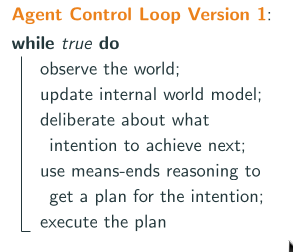
\includegraphics[scale=0.65]{03/agent1.png}
    \caption{Una prima versione di un agente che utilizza il pratical reasoning.}
\end{figure}

\paragraph{Nella prima versione:}

\begin{itemize}
  \item I processi di deliberation e means-end reasoning non sono immediati, hanno un costo nel tempo.
  \item Supponiamo che l'agente inizi a deliberare all'istante $t_0$, inizi il means-end reasoning all'istante $t_1$ e che cominci l'esecuzione del piano all'istante $t_2$: 
    \begin{itemize}
      \item Il tempo per deliberare è $t_d= t_1 - t_0$. 
    \item Il tempo per il means-end reasoning è $t_{me} = t_2 - t_1$. 
    \item Supponiamo inoltre che la deliberazione sia ottimale, cioè se si seleziona un'intenzione da raggiungere essa sia la migliore per l'agente. 
    \item Al tempo $t_1$ l'agente ha selezionato l'intenzione da raggiungere che sarebbe stata ottimale se fosse stata raggiunta all'istante $t_0$.
      \item A meno che $t_d$ sia molto piccolo c'è il rischio che l'intenzione non sia più ottimale (calculative rationality). 
    \end{itemize}
\end{itemize}

\paragraph{L'agente avrà un comportamento complessivo ottimale nelle seguenti circostanze:}

\begin{itemize}
  \item Quando il tempo impiegato per i processi di deliberazione di means-end è estremamente piccolo. 
  \item Quando il mondo è \fancyglitter{statico} mentre l'agente effettua o suoi processi. 
  \item Quando un'intenzione ottimale se raggiunta al tempo $t_0$ (il momento in cui si osserva il mondo) è garantita rimanere ottimale fino al tempo $t_2$ (il tempo in cui l'agente ha determinato le azioni per raggiungere le intenzioni).
\end{itemize}

\begin{figure}[!h]
    \centering
    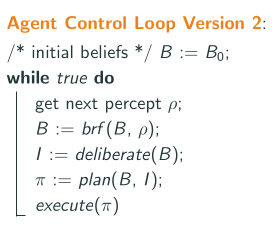
\includegraphics[scale=0.65]{03/agent2.png}
    \caption{Seconda versione di un agente che utilizza il pratical reasoning.}
\end{figure}

\paragraph{Nella seconda versione:}

\begin{itemize}
  \item $B$: credenze. 
  \item $I$: intenzioni. 
  \item $brf()$: revisione delle credenze. 
  \item $deliberate()$: deliberazione delle intenzioni. 
  \item $plan()$: pianificazione.
  \item La pianificazione è la progettazione di una sequenza di azioni che consentirà di raggiungere l'obiettivo desiderato. 
  \item Dati: 
    \begin{itemize}
      \item Una rappresentazione dell'obiettivo/intenzione da raggiungere. 
      \item Una rappresentazione delle azioni che può eseguire. 
      \item Una rappresentazione dell'ambiente.
    \end{itemize}
  \item Si tratta di automatica programming.
\end{itemize}

\qs{}{Come un agente delibera?}

\begin{itemize}
  \item \fancyglitter{Option generation}: inizia cercando di capire quali sono le opzioni a sua disposizione sulla base delle proprie informazioni e credenze. 
  \item \fancyglitter{Filtering:} sceglie tra le opzioni possibili e si impegna verso di esse. 
\end{itemize}

\nt{Le opzioni scelte sono le intenzioni.}

\begin{figure}[!h]
    \centering
    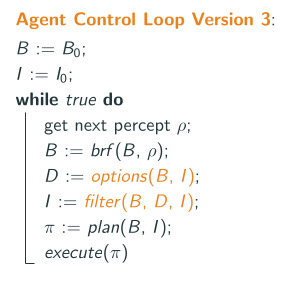
\includegraphics[scale=0.65]{03/agent3.png}
  \caption{Terza versione di un agente che utilizza il pratical reasoning.}
\end{figure}

\paragraph{Nella terza versione:}

\begin{itemize}
  \item $option()$: l'agente genera un insieme di possibili alternative. Rappresenta la generazione di opzioni tramite una funzione. 
  \item $filter()$: l'agente sceglie tra le alternative che competono e si impegna a raggiungerle. 
  \item Quando un'opzione è restituita da filter diciamo che l'agente ha fatto un \fancyglitter{commitment} verso tale opzione. 
  \item Il commitment implica persistenza temporale, per cui un'intenzione adottata non dovrebbe essere immediatamente abbandonata.
\end{itemize}

\dfn{Commitment Strategies}{
  Il meccanismo che un agente usa per determinare quando e come un'intenzione possa essere abbandonata.
}

\nt{I tipi di strategie sono gli stessi dei tipi di agente (blind, single-minded, open-minded).}

\begin{figure}[!h]
    \centering
    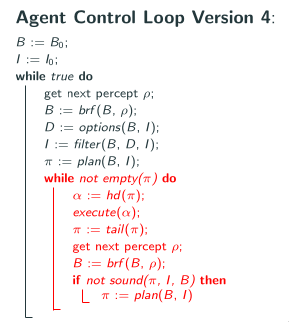
\includegraphics[scale=0.65]{03/agent4.png}
  \caption{Quarta versione di un agente che utilizza il pratical reasoning.}
\end{figure}

\paragraph{Nella quarta versione:}

\begin{itemize}
  \item Si ripianifica se qualcosa va storto. 
  \item È ancora presente overcommitment rispetto alle intenzioni: non si ferma a valutare se le sue intenzioni siano più o meno adeguate (blind). 
\end{itemize}
\pagebreak
\begin{figure}[!h]
    \centering
    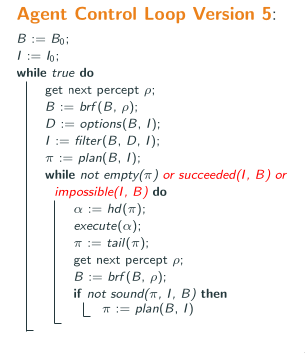
\includegraphics[scale=0.65]{03/agent5.png}
  \caption{Quinta versione di un agente che utilizza il pratical reasoning.}
\end{figure}

\paragraph{Nella quinta versione:}

\begin{itemize}
  \item Ci si ferma per determinare se le intenzioni hanno avuto successo o se sono diventate impossibili da soddisfare (single-minded). 
  \item L'agente può riconsiderare le sue intenzioni ogni volta che il controllo è sul ciclo esterno, ossia quando:
    \begin{itemize}
      \item Ha completamente eseguito un piano per raggiungere le sue intenzioni correnti. 
      \item Ritiene di aver raggiunto le sue attuali intenzioni.
      \item Crede che le sue attuali intenzioni non siano più possibili.
    \end{itemize}
  \item Questo limita il modo in cui consente a un agente di riconsiderare le sue intenzioni.
\end{itemize}
\pagebreak
\begin{figure}[!h]
    \centering
    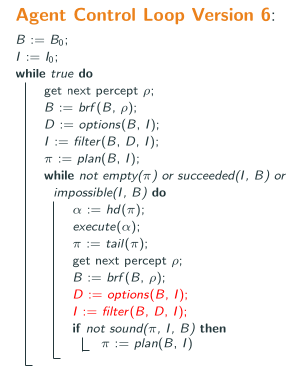
\includegraphics[scale=0.65]{03/agent6.png}
  \caption{Sesta versione di un agente che utilizza il pratical reasoning.}
\end{figure}

\paragraph{Nella sesta versione:}

\begin{itemize}
  \item Riconsidera le intenzioni dopo l'esecuzione di ogni azione (open-minded).
  \item Tuttavia la riconsiderazione delle intenzioni costa: 
    \begin{itemize}
      \item Un agente che non si ferma abbastanza spesso continuerà a tentare di raggiungere le sue intenzioni anche dopo che sarà chiaroo che non possono essere raggiunte. 
      \item Un agente che riconsidera costantemente dedica poco tempo a raggiungere le sue intenzioni.
    \end{itemize}
\end{itemize}

\begin{figure}[!h]
    \centering
    
\includegraphics[scale=0.35]{03/shinji.png}
  \caption{L'agente che riconsidera costantemente be like.}
\end{figure}

\pagebreak
\subsection{Riconsiderazione delle Intenzioni}

\begin{figure}[!h]
    \centering
    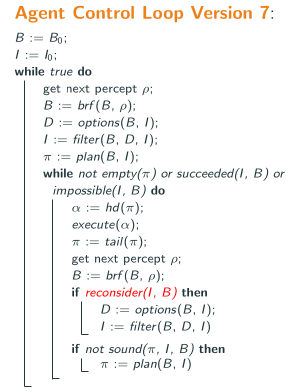
\includegraphics[scale=0.65]{03/agent7.png}
  \caption{Settima versione di un agente che utilizza il pratical reasoning.}
\end{figure}

\paragraph{Nella settima versione:}

\begin{itemize}
  \item Incorpora una componente di controllo esplicita \fancyglitter{meta-livello} che decide se eseguire o meno la riconsiderazione. 
\end{itemize}

\begin{figure}[!h]
    \centering
    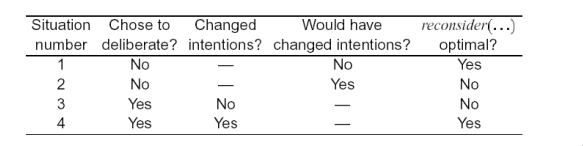
\includegraphics[scale=0.7]{03/controllo.png}
  \caption{Componente meta-livello.}
\end{figure}

\nt{Il problema è che la reconsider() è una funzione oracolo, per cui va implementata mediante euristiche e studi specifici sul dominio. Il costo di questa funzione dovrebbe essere molto inferiore al costo del processo deliberativo stesso.}

\paragraph{Kinny e Georgeff hanno investigato ciò in maniera sperimentale:}

\begin{itemize}
  \item Due tipi di agenti: 
    \begin{itemize}
      \item \fancyglitter{Bold agents}: non si fermano mai a riconsiderare le intenzioni. 
      \item \fancyglitter{Cautious agents}: riconsiderano le intenzioni dopo ogni azione.
    \end{itemize}
  \item Considerazioni:
    \begin{itemize}
      \item Se l'ambiente non cambia rapidamente gli agenti bold funzionano meglio. 
      \item Se l'ambiente cambia costantemente gli agenti cautious funzionano meglio.
    \end{itemize}
\end{itemize}

\section{Linguaggi e Architetture per Agenti}

\subsection{Procedural Reasoning System}

\dfn{PRS}{
  Il procedural reasoning system è stata una delle prime architetture per agenti che abbia fatto uso del paradigma BDI. È stata usata in applicazioni multi-agenti. 
}

\begin{figure}[!h]
    \centering
    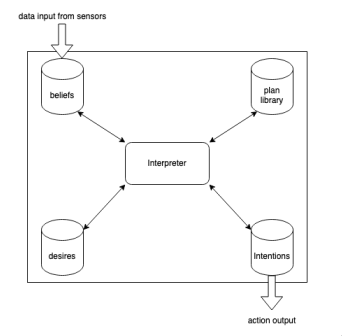
\includegraphics[scale=0.7]{03/PRS.png}
  \caption{Procedural Reasoning System.}
\end{figure}

\clm{}{}{\begin{itemize}
  \item Gli input del sistema sono \fancyglitter{eventi}, ricevuti attraverso una \fancyglitter{coda di eventi}. 
  \item Gli eventi possono essere: 
    \begin{itemize}
      \item \fancyglitter{Esterni}: percepiti dall'ambiente. 
      \item \fancyglitter{Interni}: come aggiunta o cancellazione di belief o goal.
    \end{itemize}
  \item Gli output sono azioni che sono eseguite dall'interprete. 
  \item I belief sono rappresentati come fatti del Prolog (atomi della logica del primordine). 
  \item In PRS gli agenti non pianificano, ma fanno riferimento a una libreria di piani predefinita dal programmatore.
\end{itemize}
}

\paragraph{I componenti di un piano sono:}

\begin{itemize}
  \item \fancyglitter{Nome}. 
  \item \fancyglitter{Condizioni di invocazione}. 
  \item \fancyglitter{Precondizioni}: le condizioni che devono valere prima di avviare l'esecuzione del piano. 
  \item \fancyglitter{Body}: una sequenza di espressioni: 
    \begin{itemize}
      \item Azioni atomiche. 
      \item Sottogoals.
    \end{itemize}
\end{itemize}

\nt{Per raggiungere un dato goal, l'agente formula l'intenzione di raggiungere l'obiettivo, cioè sceglie un piano applicabile. Questo piano diventa un'intenzione, ed è aggiunto alla intention structure.}

\paragraph{I piani in PRS:}

\begin{itemize}
  \item I goal in PRS possono essere complessi e contenere a loro volta dei goal. 
  \item I piani possono contenere disgiunzioni di goal, loops, etc.
  \item Un agente ha un insieme di piani, alcuni belief iniziali riguardo il mondo e un goal iniziale.
  \item I belief sono rappresentati Prolog-like. 
\end{itemize}

\paragraph{Ragionamento:}

\begin{itemize}
  \item Per raggiungere un dato goal, l'agente formula l'intenzione di raggiungerlo (sceglie un piano applicabile). Il piano diventa un'intenzione ed è aggiunto alla intention structure. 
  \item A ogni passo del loop principale, l'interprete sceglie un piano (parzialmente eseguito) nella intention structure e ne esegue un passo. 
  \item Se ci sono molte opzioni disponibili l'interprete può scegliere quella con la massima utilità o entrare in un ragionamento di meta-livello.
\end{itemize}

\paragraph{Control loop:}

\begin{enumerate}
  \item Aggiorna belief e goal secondo gli eventi della \fancyglitter{event queue}. 
  \item I cambiamenti dei goal e dei belief fanno scattare i diversi piani.
  \item Uno o più piani applicabili sono scelti e messi nella intention structure. 
    \item Si sceglie una intenzione (task) dalla intention structure. 
    \item Si esegue un passo di quel task: 
      \begin{itemize}
        \item Esecuzione di un'\fancyglitter{azione primitiva}. 
        \item Scelta di un nuovo subgoal.
      \end{itemize}
\end{enumerate}

\paragraph{Stack delle intenzioni:}

\begin{itemize}
  \item Quando un agente inizia la sua esecuzione, il goal iniziale è inserito nell'intention stack. 
  \item Lo stack contiene tutti i goal in attesa di essere soddisfatti. 
  \item L'agente cerca tra i suoi piani per vedere quali hanno un goal sulla cima dello stack delle intenzioni come la loro post-condizione. 
  \item Tra questi piani alcuni avranno le loro precondizioni soddisfatte dall'insieme di belief correnti.
  \item L'insieme dei piani che permettono di raggiungere il goal e hanno le precondizioni soddisfatte diventano l'insieme delle possibili opzioni dell'agente.
\end{itemize}

\clm{}{}{
  \begin{itemize}
    \item Il processo di selezione tra i diversi piani è la \fancyglitter{deliberazione}. 
    \item La deliberazione è ottenuta mediante l'utilizzo di un piano metà meta-livello. 
    \item Effettuata la scelta la sua esecuzione può portare ulteriori goal nello stack. 
    \item Le azioni atomiche potranno essere eseguite direttamente dall'agente. 
    \item Se un piano fallisce, l'agente può selezionare un nuovo piano tra quelli candidati. 
    \item L'esecuzione dei task può essere \fancyglitter{interleaved} (supporta il multithread). 
    \item Le intenzioni (task) sono solitamente implementate con uno stack di frames.
  \end{itemize}
}


\dfn{AgentSpeak(L)}{
 Il linguaggio AgentSpeak(L) è stato proposto come linguaggio di programmazione per agenti (BDI) e consente di essere scritto e interpretato in modo simile a quello dei programmi logici basati su clausole di Horn (Prolog). 
}

\nt{Si propone di colmare il gap tra specifica teorica e implementazione di un agente BDI. Ha dato origine a JASON.}

\subsection{Agent-Oriented Programming}

L'articolo Agent-Oriented programming di Shoham propone un nuovo paradigma di programmazione che promuove una visione sociale della computazione in cui più agenti interagiscono l'uno con l'altro. L'articolo presenta:
\begin{itemize}
  \item Un linguaggio formale per descrivere stati mentali. 
  \item Un linguaggio di programmazione per definire agenti. 
\end{itemize}

\paragraph{Caratteristiche:}

\begin{itemize}
  \item Ci sono due categorie mentali principali: \fancyglitter{belief} e \fancyglitter{obligation}. Un'ulteriore categoria, che non è un costrutto mentale, è \fancyglitter{capability}. 
  \item \fancyglitter{Decision} è una obligation a se stessi. 
  \item Le formule fanno esplicitamente riferimento al tempo. Viene adottato un semplice linguaggio basato sugli istanti di tempo. 
  \item Le azioni non sono distinte dai fatti: la presenza di un'azione è rappresentata dal fatto corrispondente.
\end{itemize}

\nt{Il linguaggio di Shoham, Agent0, non ha avuto molta rilevanza, contrariamente al nome Agent-Oriented Programming.}

\subsection{Agenti Reattivi}

\nt{Un linguaggio per agenti reattivi è CLIPS, visto in "Intelligenza Artificiale e Laboratorio".}

\paragraph{Tesi di Brooks:}

\begin{itemize}
  \item Un comportamento intelligente può essere generato \fancyglitter{senza rappresentazione esplicita} del tipo di ciò che è proposto dall'IA simbolica. 
  \item  Un comportamento intelligente può essere generato \fancyglitter{senza ragionamento esplicito} del tipo di ciò che è proposto dall'IA simbolica. 
  \item L'intelligenza è una proprietà \fancyglitter{emergente} di certi sistemi complessi.
\end{itemize}

\paragraph{Due idee chiave:}

\begin{itemize}
  \item \fancyglitter{Collocazione e personificazione}: l'intelligenza reale è situata nel mondo, non in sistemi senza sostanza come i "theorem provers" o i "sistemi esperti"\footnote{AKA touch some grass.}. 
  \item \fancyglitter{Intelligenza e apparenza}: il comportamento intelligente è generato come un risultato di un'interazione con l'ambiente.
\end{itemize}

\dfn{Subsumption Architecture}{
  Una Subsumption Architecture è una gerarchia di task che eseguono behaviours.
}

\cor{Behaviour}{
  Una behaviour è una struttura a regole molto semplici. 
}

\paragraph{Subsumption Architecture:}
\begin{itemize}
  \item Ogni behaviours compete con altri per esercitare il controllo sugli agenti. 
  \item Gli strati più bassi rappresentano tipi di behaviours più primitivi e hanno precedenza su strati più in alto nella gerarchia. 
  \item I sistemi risultanti sono estremamente semplici in termini della quantità di computazione che fanno. 
  \item Alcuni robot eseguono task che sarebbero sconvolgenti se eseguiti da sistemi simbolici di AI.
\end{itemize}

\paragraph{Selezione delle azioni:}

\begin{itemize}
  \item La scelta di un'azione è realizzata mediante insiemi di behaviours (coppie $(c, a)$):
    \begin{itemize}
      \item $c$: insieme di \fancyglitter{condizioni}. 
      \item $a$: un'azione.
    \end{itemize}
  \item Un behaviour scatta quando la funzione $see$ restituisce una percezione $p$ tale che $p \in c$. 
  \item Associato a un insieme di behaviour rules c'è una \fancyglitter{relazione di inibition}. 
  \item Leggiamo $b_1 < b_2$ come "$b_1$ inibisce $b_2$", cioé $b_1$ è più basso nella gerarchia di $b_2$, quindi ha priorità.
\end{itemize}

\dfn{Steels Mars Explorer}{
  Steels propose un sistema di esplorazione per Marte usando la Subsumption Architecture. La soluzione fa uso di due meccanismi:
  \begin{itemize}
    \item Un campo gradiente per trovare la direzione verso la base. 
    \item "Briciole radioattive" per permettere la comunicazione tra agenti. 
  \end{itemize}
}

\paragraph{Regole non-cooperative:}

\begin{enumerate}
  \item Evitare gli ostacoli. 
  \item I campioni portati dagli agenti sono depositati alla base. 
  \item Gli agenti che portano i campioni ritornano alla base. 
  \item Gli agenti raccolgono i campioni che trovano. 
  \item Un agente che non sa cosa fare esplora a caso.
\end{enumerate}

\clm{}{}{
  \begin{itemize}
    \item Si vuole favorire la collaborazione. 
    \item Un agente crea un sentiero di briciole radioattive ogni volta che trova un campione di roccia. 
    \item Il sentiero sarà creato quando un agente riporta le rocce alla base. 
    \item Mentre un agente segue un sentiero verso la sorgente di rocce, raccoglie le briciole rendendo il sentiero più sottile. 
    \item Dopo che un po' di agenti avranno seguito il sentiero senza trovare campioni il sentiero sarà scomparso.
  \end{itemize}
}

\paragraph{Viene rimossa la regola tre e aggiunte:}

\begin{itemize}
  \item [6.] Se un agente sta portando dei campioni e non è nella base, lascia cadere 2 briciole e va su verso il gradiente. 
  \item [7.] Se un agente percepisce delle briciole ne prende una e va giu verso il gradiente.
\end{itemize}

\nt{L'ordine dei behaviours è 1, 2, 6, 4, 7, 5.}

\paragraph{Limiti degli agenti reattivi:}

\begin{itemize}
  \item Agenti senza modello devono avere sufficienti informazioni locali. 
  \item Se le decisioni sono locali gli agenti hanno una visione a breve termine. 
  \item Difficili da realizzare. 
    \item È difficile ingegnerizzare agenti specifici. 
    \item È difficile definire agenti con un gran numero di behaviours.
\end{itemize}

\subsection{Architetture Ibride}

\begin{itemize}
  \item Molti ricercatori hanno sostenuto che né un approccio completamente deliberativo né un approccio completamente reattivo sono adatti a costruire agenti. 
  \item Ci sono stati suggerimenti di utilizzo di sistemi ibridi. 
  \item Un approccio è quello di costruire un agente con due o più sottosistemi:
    \begin{itemize}
      \item Uno \fancyglitter{deliberativo} contenente un modello simbolico del mondo, che sviluppa piani e prende decisioni nel modo proposto dall'IA simbolica. 
      \item Uno \fancyglitter{reattivo} capace di reagire a eventi senza ragionamenti complessi.
    \end{itemize}
\end{itemize}

\paragraph{Modelli ibridi:}

\begin{itemize}
  \item Solitamente viene data precedenza ai componenti reattivi. 
  \item Questo tipo di struttura porta a un'architettura a strati. 
  \item I sottosistemi di controllo di un agente sono organizzati in una gerarchia, con livelli più alti che trattano l'informazione a crescenti livelli di astrazione. 
  \item Un problema è il tipo di schema di controllo in cui inserire i sottosistemi. 
  \item Sono stati proposti:
    \begin{itemize}
      \item \fancyglitter{Horizontal layering:} tutti gli strati sono direttamente connessi all'input e all'output. 
      \item \fancyglitter{Vertical layering:} input dei sensori e output delle azioni sono gestiti al massimo da uno strato ciascuno.
    \end{itemize}
\end{itemize}

\begin{figure}[!h]
    \centering
    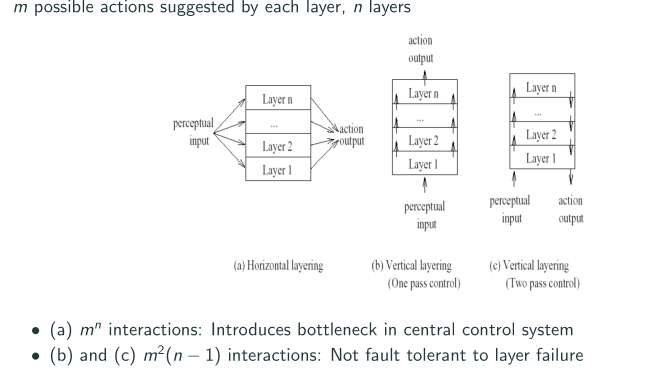
\includegraphics[scale=0.7]{03/archybr.png}
  \caption{Schema delle architetture ibride.}
\end{figure}

\nt{Esempi di architetture ibride sono TOURINGMACHINES e Stanley.}






